%!TEX root = ../main.tex

\par
A hurricane is one of the most destructive weather events in the United States.
Every fall, major storms threaten states along the Gulf Coast and Atlantic ocean with high winds, heavy rain, and storm surge.
Some hurricanes proceed to make landfall, causing significant damage to life and property, while others avoid land altogether, having almost zero human impact.
So understandably, the modeling and prediction of Atlantic hurricanes is an important topic of study.
The goal of this paper is to present a statistical method of estimating the probability that a hurricane makes landfall based on its formation and early motion.

\par
In this paper, I will begin by presenting the revised Atlantic hurricane database, called HURDAT2~(\cite{landsea2015revised}), which will provide the data used for our algorithms.
I will discuss some of the key variables within the data that my analysis will focus on, provide some high-level information about the data, and briefly look at how I process the data into my code.
Next, I will present the prediction method.
I will discuss the time series similarity metrics presented by~\cite{ho2015manifold}, and explain how I use them to perform dimension reduction on the set of hurricane tracks.
I then explain how I compute a local linear kernel regression esimate of the projected data, with respect to whether or not a storm made landfall.
I also mention the procedure for using the learned model to predict whether or not a hurricane will make landfall.
At this point, I will also compare methods of generating new hurricane data, and perform some basic analysis to demonstrate that the generated data is realistic.
I will then perform a full analysis demonstrating the strengths and weaknesses of my method.
The paper will conclude with a brief discussion on the implications of my work, and directions of future research.

\begin{figure}
	\centering
	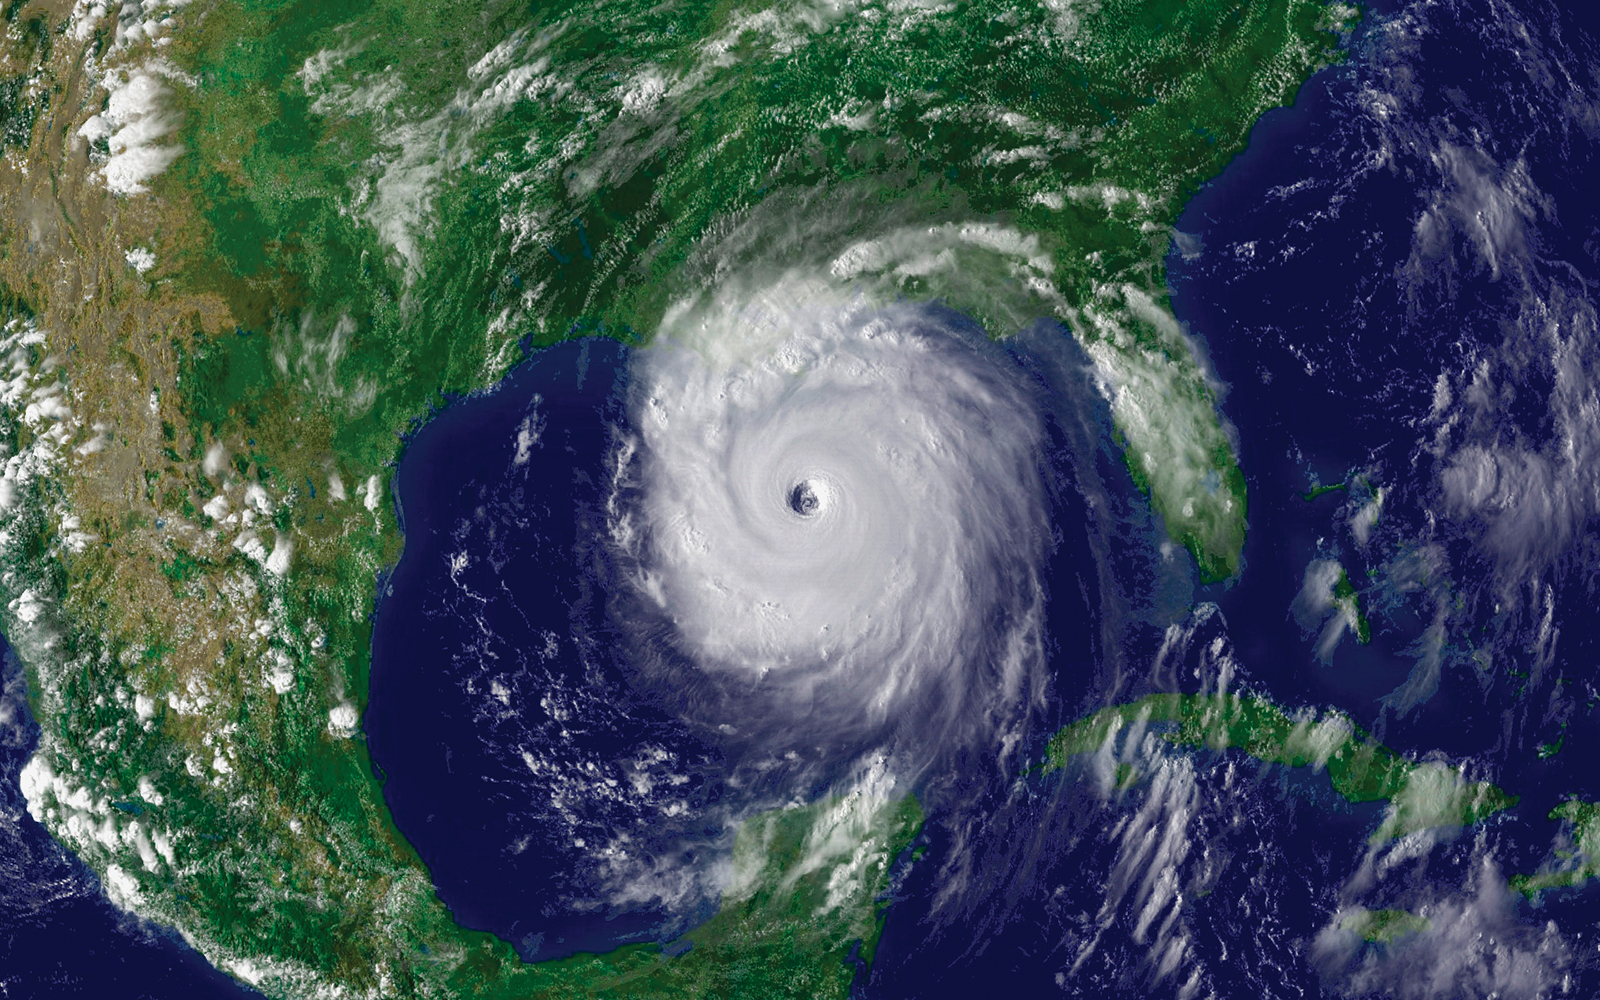
\includegraphics[width=\linewidth]{images/katrina_satellite_noaa.jpg}
	\caption{A satellite image of Hurricane Katrina, taken in 2005. Over 1200 people were killed, and the storm did over \$160 billion dollars of damage. \textit{NOAA}}
	\label{fig:katrina_satellite}
\end{figure}

\begin{figure}
	\centering
	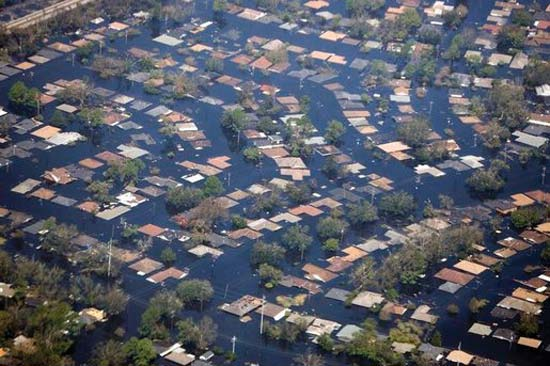
\includegraphics[width=\linewidth]{images/katrina_flooding_paul_morse.jpg}
	\caption{A flooded neighborhood of New Orleans, in the aftermath of Hurricane Katrina. \textit{Paul Morse}}
	\label{fig:katrina_flooding}
\end{figure}